\documentclass[12pt]{article}
\usepackage{graphicx}			    % Use this package to include images %Path relative to the main .tex file 
\graphicspath{ {./Images/} }
\usepackage{amsmath}			    % A library of many standard math expressions
\usepackage{mathtools}              % For Aboxed{} (https://tex.stackexchange.com/questions/346577/boxed-and-align)
% \usepackage[margin=1in]{geometry} % Sets 1in margins. 
\usepackage{fancyhdr}			    % Creates headers and footers
\usepackage{enumerate}              % These two packages give custom labels to a list
\usepackage[shortlabels]{enumitem}
\usepackage{hyperref}               % https://www.overleaf.com/learn/latex/Hyperlinks
\usepackage{xcolor}
\usepackage[svgnames]{xcolor}
\usepackage{float}
\usepackage{cmupint}                % For upright integrals. https://tex.stackexchange.com/questions/503527/how-to-write-upright-integrals-with-automatic-sizing
\usepackage{tikz}
\usetikzlibrary{trees}
\usepackage{titling}
\usepackage{minted}                 % For code blocks
\usemintedstyle{monokai}            % For code blocks
\definecolor{bg}{HTML}{282828}      % For code blocks, from https://github.com/kevinsawicki/monokai
\usepackage{nameref}
\usepackage{caption}                % To use \caption*{} to show only the caption text without "Table 1: <text>"
\usepackage[main,largesymbols]{tccomicsans} % https://www.reddit.com/r/LaTeX/comments/1l5no5d/comment/mwm64ze/
\renewcommand*\contentsname{Summary}
% \renewcommand{\contentsname}{\centering \normalfont\normalsize Contents}
\renewcommand{\contentsname}{\centering \bfseries\Large Contents}
% \renewcommand{\cftaftertoctitle}{\hfill}

\hypersetup
{
    colorlinks=true,
    linkcolor=blue,
    filecolor=magenta,      
    urlcolor=cyan,
    %pdftitle={Overleaf Example},
    pdfpagemode=FullScreen,
}

% \title{OOP Lab Manual 05}
% \author{STM}
% \date{December 2024}

\begin{document}

\begin{titlepage}
    \centering

    \vspace*{-8em}
    
\includegraphics[width=0.5\textwidth]{Bismillah.png}%\\[2cm]
    \vspace*{5em}

    
    \vspace*{1cm}

     
\includegraphics[width=0.5\textwidth]{GU Tech 1685x1330.png}\\[2cm]

    \MakeUppercase{\Huge \textbf{GU TECH}}\\[1.5ex]
    
    \vspace*{1cm}
    
    \Huge Object Oriented Programming \\[1.5ex]
    \LARGE Lab 12 \\[2cm]

    % {\Large STM} \\ [2cm]

    {\Large \today}\\[1cm]
    
\end{titlepage}

\newpage

% \vspace*{4cm}
% \begin{center}
%     \Huge \textbf{Outline}
% \end{center}

% \begin{itemize}
%    \item \nameref{Functions}
% \end{itemize}

\tableofcontents

\newpage
\addcontentsline{toc}{part}{STL Containers}
\part*{\centering STL Containers}

\noindent Recommended reading: \href{https://www.w3schools.com/cpp/cpp_data_structures.asp}{C++ Data Structures and STL} \\

\noindent C++ Standard Template Library (STL) containers are template classes that provide various data structures for storing and organizing collections of objects. They offer efficient ways to manage 
data and are categorized into three main types:

\begin{enumerate}
    \item \textbf{Sequence containers:} These containers store elements in a linear order, allowing sequential access.
    
    \begin{itemize}
        \item \textcolor{red}{\texttt{std::vector}}: A dynamic array that can grow or shrink in size. Offers fast random access and efficient additions and deletions at the end. Additions 
        and deletions in the middle are inefficient.
        \item \textcolor{red}{\texttt{std::deque}}: A \textbf{double-ended queue} that allows efficient insertions and deletions at \textbf{both} ends. Allows random access.
        \item \textcolor{red}{\texttt{std::list}}: A doubly linked list that provides efficient insertions and deletions anywhere. \textbf{No} random access.
        \item \textcolor{red}{\texttt{forward\_list}}: A singly linked list, more memory-efficient than \textcolor{red}{\texttt{std::list}} but only allows forward traversal.
        \item \textcolor{red}{\texttt{array}}: A fixed-size array that wraps a C-style array, providing bounds checking and other utility functions.
    \end{itemize}

    \item \textbf{Associative containers:} These containers store elements in a linear order, allowing sequential access.

    \begin{itemize}
        \item \textcolor{red}{\texttt{std::set}}: Stores unique elements in a sorted order.
        \item \textcolor{red}{\texttt{std::multiset}}: Similar to \textcolor{red}{\texttt{std::set}} but allows duplicate elements.
        \item \textcolor{red}{\texttt{std::map}}: Stores key-value pairs, where keys are unique and sorted.
        \item \textcolor{red}{\texttt{std::multimap}}: Similar to \textcolor{red}{\texttt{std::map}} but allows duplicate keys.
    \end{itemize}

    \item \textbf{Unordered associative containers:} These containers store elements in an unordered fashion using hash tables, offering average constant-time complexity for search, insertion, and deletion.

    \begin{itemize}
        \item \textcolor{red}{\texttt{std::unordered\_set}}: Stores unique elements in an unordered fashion.
        \item \textcolor{red}{\texttt{std::unordered\_multiset}}: Similar to \textcolor{red}{\texttt{std::unordered\_set}} but allows duplicate elements.
        \item \textcolor{red}{\texttt{std::unordered\_map}}: Stores key-value pairs in an unordered fashion, where keys are unique.
        \item \textcolor{red}{\texttt{std::unordered\_multimap}}: Similar to \textcolor{red}{\texttt{std::unordered\_map}} but allows duplicate keys. 
    \end{itemize}

    \item \textbf{Container adapters:} These are not standalone containers but provide a specific interface built on top of existing containers.

    \begin{itemize}
        \item \textcolor{red}{\texttt{std::stack}}: A LIFO (Last-In, First-Out) data structure.
        \item \textcolor{red}{\texttt{std::queue}}: A FIFO (First-In, First-Out) data structure.
        \item \textcolor{red}{\texttt{std::priority\_queue}}: A queue where elements are retrieved based on their priority.
    \end{itemize}

\end{enumerate}

\newpage
\begin{table}[H]
\makebox[\linewidth][c]
{
    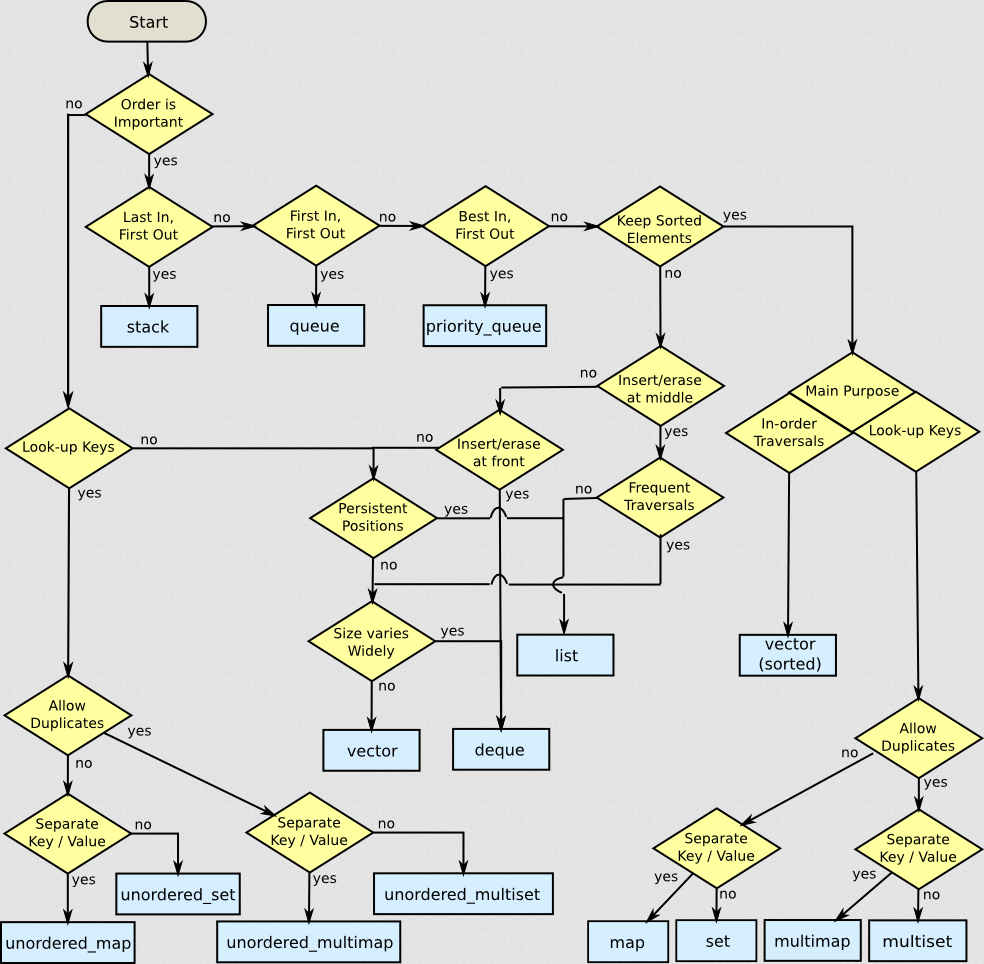
\includegraphics[scale=0.8]{chart}
}
\end{table}
\newpage

\noindent Chart source: \href{https://stackoverflow.com/questions/471432/in-which-scenario-do-i-use-a-particular-stl-container}{Stackoverflow}

\addcontentsline{toc}{section}{Vectors}
\section*{Vectors}

\noindent \textcolor{red}{\texttt{std::vector}} is the most used data structure and is typically used as a replacement for arrays.

\begin{itemize}
    \item It lets us add elements without specifying the number of elements beforehand. 
    \item It allows random access (by using subscript \textcolor{red}{\texttt{[]}} or \textcolor{red}{\texttt{.at()}} function).
    \item Unlike arrays, it allows insertion and deletion in the middle but it is extremely inefficient to do so.
    \begin{itemize}
        \item On insertion, all succeeding elements are shifted forward.
        \item On deletion, all succeeding elements are shifted backward.
    \end{itemize}
\end{itemize}

\noindent For comparision, an \textcolor{red}{\texttt{std::list}} allows efficient insertions and deletions in the middle as well but does not allow random access. The access has to be 
sequential.

\newpage
\addcontentsline{toc}{subsection}{Vector Usage}
\subsection*{Vector Usage}

\noindent Before we can use vectors or other STL containers, we need to include their respective headers. 

\begin{minted}[bgcolor=bg, framesep=2mm]{cpp}
#include <iostream>
#include <vector>
using namespace std;

void main()
{
    vector<int> equation;   //3x^2 + 2x^1 - 8x^0 = 0
    equation.push_back(3);
    equation.push_back(2);
    equation.push_back(-8);

    for (int i = 0; i < equation.size(); i++)
    {
        cout << equation[i] << " ";
    }
    cout << "\n";

    for (int i = 0; i < equation.size(); i++)
    {
        cout << equation.at(i) << " ";
    }
    cout << "\n";
}
\end{minted}

\newpage

\noindent It is important to note that STL \textcolor{red}{\texttt{pop()}} functions do not return values.

\begin{minted}[bgcolor=bg, framesep=2mm]{cpp}
#include <iostream>
#include <vector>
using namespace std;

void main()
{
    vector<int> equation;
    //9x^4 + 12x^3 - 44x^2 - 32x^1 + 64x^0 = 0
    equation.push_back(9);
    equation.push_back(12);
    equation.push_back(-44);
    equation.push_back(-32);
    equation.push_back(64);

    for (int i = 0; i < equation.size(); i++)
    {
        cout << equation[i] << " ";
        //9 12 -44 -32 64
    }
    cout << "\n";

    //  cout << equation.pop_back() << "\n"; //Error
    equation.pop_back();

    for (int i = 0; i < equation.size(); i++)
    {
        cout << equation[i] << " ";
        //9 12 -44 -32
    }
    cout << "\n";
}
\end{minted}

\newpage

\noindent The follwoing code demonstrates insertion and deletion in the middle. \\

\noindent \textbf{Reminder:} Insertion and deletion in the middle of a vector are extremely inefficient.

\begin{minted}[bgcolor=bg, framesep=2mm]{cpp}
#include <iostream>
#include <vector>
using namespace std;

void printVector(vector<int> v)
{
    for (int i = 0; i < v.size(); i++)
    {
    	cout << v[i] << " ";
	}
	cout << "\n";	
}

int main()
{
    vector<int> numbers = {0, 1, 2, 3, 4};

    printVector(numbers);
    //0 1 2 3 4
    numbers.insert(numbers.begin() + 2, 5);
    printVector(numbers);
    //0 1 5 2 3 4
    numbers.erase(numbers.begin() + 2);
    printVector(numbers);
    //0 1 2 3 4

    //numbers.insert(2, 5); //Does not work
    //numbers.erase(2);     //Does not work

    return 0;
}
\end{minted}

\newpage
\addcontentsline{toc}{section}{Runtime Polymorphism with STL Containers}
\section*{Runtime Polymorphism with STL Containers}

\begin{minted}[bgcolor=bg, framesep=2mm]{cpp}
#include <iostream>
#include <vector>
using namespace std;

class Animal
{ public: virtual void speak(){cout << "gibberish\n";} };

class Cat : public Animal
{ public: void speak(){cout << "Meow\n";} };

class Dog : public Animal
{ public: void speak(){cout << "Woof\n";} };

int main()
{
    vector <Animal*> jungle;
    jungle.push_back(new Cat());
    jungle.push_back(new Dog());
    jungle.push_back(new Cat());

    for (int i = 0; i < jungle.size(); i++)
    {
        jungle[i]->speak();
    }

    for (int i = 0; i < jungle.size(); i++)
    {
        delete jungle[i];
    }

    return 0;
}
\end{minted}

\noindent \textbf{Reminder:} Every single \textcolor{red}{\texttt{new}} should have a corresponding \textcolor{red}{\texttt{delete}} and every single \textcolor{red}{\texttt{new[]}} should 
have a corresponding \textcolor{red}{\texttt{delete[]}}. \\

\newpage
\addcontentsline{toc}{section}{Iterating through STL Containers}
\section*{Iterating through STL Containers}

\begin{itemize}
    \item STL containers that allow random access may be iterated with \textcolor{red}{\texttt{for}} loops using the \textcolor{red}{\texttt{.size()}} function, just like iterating regular arrays.
        
    \begin{itemize}
        \item These containers include \textcolor{red}{\texttt{std::vector}}, \textcolor{red}{\texttt{std::deque}} and \textcolor{red}{\texttt{std::array}}. 
        \item \textcolor{red}{\texttt{std::array}} should not be confused with regular arrays.
    \end{itemize}

    \item All iterable containers can be iterated with \textcolor{red}{\texttt{for each}} loops, (not to be confused with \textcolor{red}{\texttt{std::for\_each}} loop).
    
    \begin{itemize}
        \item This includes iterating by value and iterating by reference.
    \end{itemize}

    \item All iterable containers can also be iterated with \textcolor{red}{\texttt{iterators}}.

    \item \textcolor{red}{\texttt{std::stack}} and \textcolor{red}{\texttt{std::queue}} cannot be iterated at all (by design).

    \item The \textcolor{red}{\texttt{std::for\_each}} loop from the \textcolor{red}{\texttt{<algorithm>}} header may also be used for all iterable containers but this manual does not cover that.

\end{itemize}

\newpage
\addcontentsline{toc}{subsection}{Iterating with For Loops}
\subsection*{Iterating with For Loops}

\begin{minted}[bgcolor=bg, framesep=2mm]{cpp}
#include <iostream>
#include <vector>
#include <deque>
using namespace std;

int main()
{
    vector<int> numbers = {0, 1, 2, 3, 4};
    deque<string> words = 
    {"comic", "sans", "reigns", "supreme"};

    for (int i = 0; i < numbers.size(); i++)
    {
        cout << numbers[i] << " ";
    }
    cout << "\n";

    for (int i = 0; i < words.size(); i++)
    {
        cout << words[i] << " ";
    }
    cout << "\n";

    return 0;
}
\end{minted}

\newpage
\addcontentsline{toc}{subsection}{Iterating with For Each Loops}
\subsection*{Iterating with For Each Loops}

\begin{minted}[bgcolor=bg, framesep=2mm]{cpp}
#include <iostream>
#include <vector>
using namespace std;

int main()
{
    vector<int> numbers = {0, 1, 2, 3, 4};

    for (const int i : numbers)
    {
        cout << i << " ";
        //0 1 2 3 4
    }
    cout << "\n";

    for (int& i : numbers)
    {
        i = i * i;
    }

    for (const int i : numbers)
    {
        cout << i << " ";
        //0 1 4 9 16
    }
    cout << "\n";

    return 0;
}
\end{minted}

\newpage

\noindent When iterating STL containers where each element holds a single data type, we can simply use a variable of that data type in our \textcolor{red}{\texttt{for each}} loop. \\

\noindent For example, when iterating \textcolor{red}{\texttt{vector<int> numbers = {0, 1, 2, 3, 4}}}, we can simply use \textcolor{red}{\texttt{for (int i : numbers)}}. \\

\noindent However, for STL containers that contain a pair of values, we need to use \textcolor{red}{\texttt{for (std::pair<data\_type\_1, data\_type\_2> i) : containerName}}. 

\begin{minted}[bgcolor=bg, framesep=2mm]{cpp}
#include <iostream>
#include <map>
using namespace std;

int main()
{	
    map<string, string> students =
                     {{"K164078", "KMT"}, 
                      {"K163859", "SMR"}, 
                      {"K163860", "STM"}};

    for (std::pair<string, string> i : students)
    {
        cout << i.first << ", " 
             << i.second << "\n";
    }

    return 0;
}
\end{minted}

\vspace{1cm}

\noindent \textbf{Note:} When using associative containers, the \textcolor{red}{\texttt{<}} operator is used by default for sorting. This implies that when custom classes are used with 
associative containers, the \textcolor{red}{\texttt{<}} operator should be overloaded. \\

\noindent Associative containers store elements in a sorted order. \\





\newpage
\addcontentsline{toc}{subsection}{Iterating with Iterators}
\subsection*{Iterating with Iterators}

\begin{minted}[bgcolor=bg, framesep=2mm]{cpp}
#include <iostream>
#include <vector>
using namespace std;

int main()
{
    vector<int> numbers = {0, 1, 2, 3, 4};

    for (vector<int>::iterator it = 
        numbers.begin(); 
        it != numbers.end(); it++)
    {
        cout << *it << " ";
        //0 1 2 3 4
    }
    cout << "\n";

    for (vector<int>::reverse_iterator rit = 
        numbers.rbegin(); 
        rit != numbers.rend(); rit++)
    {
        cout << *rit << " ";
        //4 3 2 1 0
    }
    cout << "\n";	

    return 0;
}
\end{minted}

\vspace{1cm}

\noindent Also see: \url{https://cplusplus.com/reference/vector/vector/rbegin/}


\newpage
\addcontentsline{toc}{section}{Polynomials with Vectors}
\section*{Polynomials with Vectors}

\addcontentsline{toc}{subsection}{Representation}
\subsection*{Representation}

\begin{align*}
    3x^2 + 2x + 1 &= 0 \\ 
\end{align*}

\begin{align*}
    3x^2 + 2x + 1 &= 3x^2 + 2x^1 + 1x^0 \\ 
\end{align*}

\noindent Here 3, 2 and 1 are the coefficients, and the degree of polynomial is 2. \\

\noindent We can simply store the coefficients in our array or vector, without  worrying about storing powers of x. \\

\noindent For an equation where a middle term is $0$, we will simply store a $0$. \\

\begin{align*}
    4x^3 + 2x + 1 &= 4x^3 + 0x^2 + 2x + 1 \\ 
    4x^3 + 2x + 1 &= 4x^3 + 0x^2 + 2x^1 + 1x^0 \\ 
\end{align*}











% \newpage
\addcontentsline{toc}{subsection}{Addition}
\subsection*{Addition}

\noindent Addition between two polynomials is simple. It has three cases but they are easy to handle. The cases are: 
when both polynomials have the same degree (same number of terms), when the polynomial on the left of positive sign 
has a larger degree, and when the polynomial on the right side of the positive sign has a larger degree. \\

\noindent THe first case is simple enough. \\

\noindent The last two cases require that the resultant polynomial be initiated with values (coefficients) of the greater 
polynomial. We then loop through the smaller polynomial to add like terms (terms with the same power). \\

\begin{align*}
    \intertext{Case 1:} 
    & 3x^2 + 2x^1 + 1x^0 \\
    + & 3x^2 + 2x^1 + 1x^0 \\
    \intertext{Case 2:} 
    4x^3 + & \, 3x^2 + 2x^1 + 1x^0 \\
    & \, 3x^2 + 2x^1 + 1x^0 \\
    \intertext{Case 3:} 
    & \, 3x^2 + 2x^1 + 1x^0 \\
    4x^3 + & \, 3x^2 + 2x^1 + 1x^0 \\
\end{align*}










\newpage
\addcontentsline{toc}{subsection}{Subtraction}
\subsection*{Subtraction}

\noindent As with addition, subtraction also has the same three cases, but the third case is handled differently and may seem 
unintuitive. \\

\begin{align*}
    \intertext{Case 1:} 
    & 3x^2 + 2x^1 + 1x^0 \\
    - & (3x^2 + 2x^1 + 1x^0) \\
    \intertext{Case 2:} 
    4x^3 + & \, 3x^2 + 2x^1 + 1x^0 \\
    - \, (& \, 3x^2 + 2x^1 + 1x^0 ) \\
    \intertext{Case 3:} 
    & \, 3x^2 + 2x^1 + 1x^0 \\
    - \, (4x^3 + & \, 3x^2 + 2x^1 + 1x^0) \\
    \intertext{It resolves to} 
    & \, 3x^2 + 2x^1 + 1x^0 \\
    + \, (-4x^3 - & \, 3x^2 - 2x^1 - 1x^0) \\
    \intertext{Or}
    -4x^3 \, - & 3x^2 - 2x^1 - 1x^0 \\
    + \, & 3x^2 + 2x^1 + 1x^0 \\
\end{align*}

\noindent That is, the subtraction becomes addition in this case. \\

\noindent In other words, the third subtraction case becomes the second addition case. \\










\newpage
\addcontentsline{toc}{subsection}{Multiplication}
\subsection*{Multiplication}

\noindent In multiplication, the product polynomial's degree is the sum of degrees of the two polynomials being 
multiplied. Note that it is \textbf{not} their product. \\

\noindent Multiplication also has the same three cases, but in my opinion, they are a lot easier to handle. \\

\begin{align*}
    (5x^1 + 2x^0) * (3x^2 + 2x^1 + 1x^0) &= (15x^3 + 10x^2 + 5x^0) + (6x^2 + 4x^1 + 2x^0) \\
    (5x^1 + 2x^0) * (3x^2 + 2x^1 + 1x^0) &= 15x^3 + 10x^2 + 5x^0 + 6x^2 + 4x^1 + 2x^0 \\
    (5x^1 + 2x^0) * (3x^2 + 2x^1 + 1x^0) &= 15x^3 + 16x^2 + 4x^1 + 7x^0 \\
\end{align*}

\noindent The trick with multiplication is to determine the term (power of $x$) of the product polynomial within the 
nested loops (multiplication requires that each term of one polynomial be multipled with each term of the other 
polynomial). \\






\newpage
\addcontentsline{toc}{subsection}{Long Division}
\subsection*{Long Division}

\noindent Left as an exercise to the reader...






































































\newpage
\addcontentsline{toc}{part}{Lab Tasks}
\part*{\centering Lab Tasks}

\begin{enumerate}

    \item \textbf{Library Book Catalog:} Create a \textcolor{red}{\texttt{Book}} class with appropriate constructor, getters, and the following attributes:

    \begin{itemize}
        \item \textcolor{red}{\texttt{isbn (string)}}
        \item \textcolor{red}{\texttt{author (string)}}
        \item \textcolor{red}{\texttt{title (string)}}
    \end{itemize}

    Store books in an \textcolor{red}{\texttt{unordered\_map<string, Book>}} (key = ISBN).

    Implement a \textcolor{red}{\texttt{search}} function that returns the number of books by a given author and takes a \textcolor{red}{\texttt{multimap<string, Book>}} parameter for 
    author indexing.

    \textbf{Hints:}

    \begin{itemize}
        \item You will need the following headers.
        
        \begin{itemize}
            \item \textcolor{red}{\texttt{<unordered\_map>}}
            \item \textcolor{red}{\texttt{<map>}}
        \end{itemize}

        \item Your \textcolor{red}{\texttt{search}} function can have the following prototype: 
        
        \textcolor{red}{\texttt{int search(unordered\_map<string, Book>\& library, string author, multimap<string, Book>\& searchResult)}}

        \item You can use the \textcolor{red}{\texttt{.insert()}} function for insertions. You will need to use braces inside the function, like this: 
        \textcolor{red}{\texttt{.insert(\{author, Book\})}}.

        \item Refer to the \textcolor{red}{\texttt{map}} example given in the manual for further help.
        
        \item You may consult the Internet, but do not copy code from ChatGPT.

        \item You may use the following books to test your code (you can also come up with your own). 

\begin{minted}[bgcolor=bg, framesep=2mm]{cpp}
Book b0("9635280258938", "Mercury", "Asad");
Book b1("4702599831795", "Venus", "Asad");
Book b2("8417392305289", "Earth", "Asad");
Book b3("4323267170016", "Mars", "Taimoor");
Book b4("8951093252041", "Saturn", "Unknown");
Book b5("5580166798252", "Jupiter", "Taimoor");
\end{minted}

    \end{itemize}

    \item Create a class \textcolor{red}{\texttt{Student}} with attributes \textcolor{red}{\texttt{string name}} and \textcolor{red}{\texttt{string rollNo}}. Read names and roll number 
    from a csv (or \textcolor{red}{\texttt{.txt}}) file, and store the class objects in an ordered container. Overload the \textcolor{red}{\texttt{<}} operator so that the 
    \textcolor{red}{\texttt{Student}} objects are sorted by roll numbers lexicographically, and \textbf{make sure} that the comparision is case \textbf{insensitive}. 
    
    You may use the following file for testing:

\begin{minted}[bgcolor=bg, framesep=2mm]{cpp}
24g-bCs007, hUzAiFa,
24g-bCs003, bArIrA,
24G-BcS001, Abdur Rehman,
24G-BcS002, AhSaN,
24g-bCs004, fAtImA,
\end{minted}

    \item Use \textcolor{red}{\texttt{std::stack}} to verify that a given sequence of brackets is correct 
    (all opening brackets match their closing counterparts).

    \textbf{Hint:} Iterate the string and whenever you encounter an opening bracket, push it on the stack. 
    Whenever you find a closing bracket, if it is the same type as (the one on) the top of the stack, pop the stack.

    \item Create a class \textcolor{red}{\texttt{Polynomial}} utilizing \textcolor{red}{\texttt{std::vector}} and overload the \textcolor{red}{\texttt{+}}, \textcolor{red}{\texttt{-}} and 
    \textcolor{red}{\texttt{*}} operators and preferably the \textcolor{red}{\texttt{/}} operator as well for a bonus of 2 marks. Hints to follow later.

\end{enumerate}































\end{document}
